% !TEX program = xelatex
% !TEX root = fb237_iraq_english_persian_tikz.tex
\documentclass[tikz,border=2mm]{standalone}
\usepackage[T1]{fontenc}
\usepackage{amsmath}
\usepackage[scaled=.92]{helvet}
\usepackage{tikz}
\usetikzlibrary{arrows.meta,positioning,fit,backgrounds}

\definecolor{lightblue}{RGB}{173,216,230}
\definecolor{lightgreen}{RGB}{144,238,144}
\definecolor{lightred}{RGB}{255,182,193}
\definecolor{edgegreen}{RGB}{42,135,58}
\definecolor{edgeorange}{RGB}{220,120,25}
\definecolor{edgepurple}{RGB}{135,55,150}
\definecolor{lightgray}{RGB}{240,240,240}

\newcommand{\figbody}{\fontfamily{phv}\fontseries{c}\selectfont\footnotesize}
\newcommand{\figsmall}{\fontfamily{phv}\fontseries{c}\selectfont\scriptsize}
\begin{document}
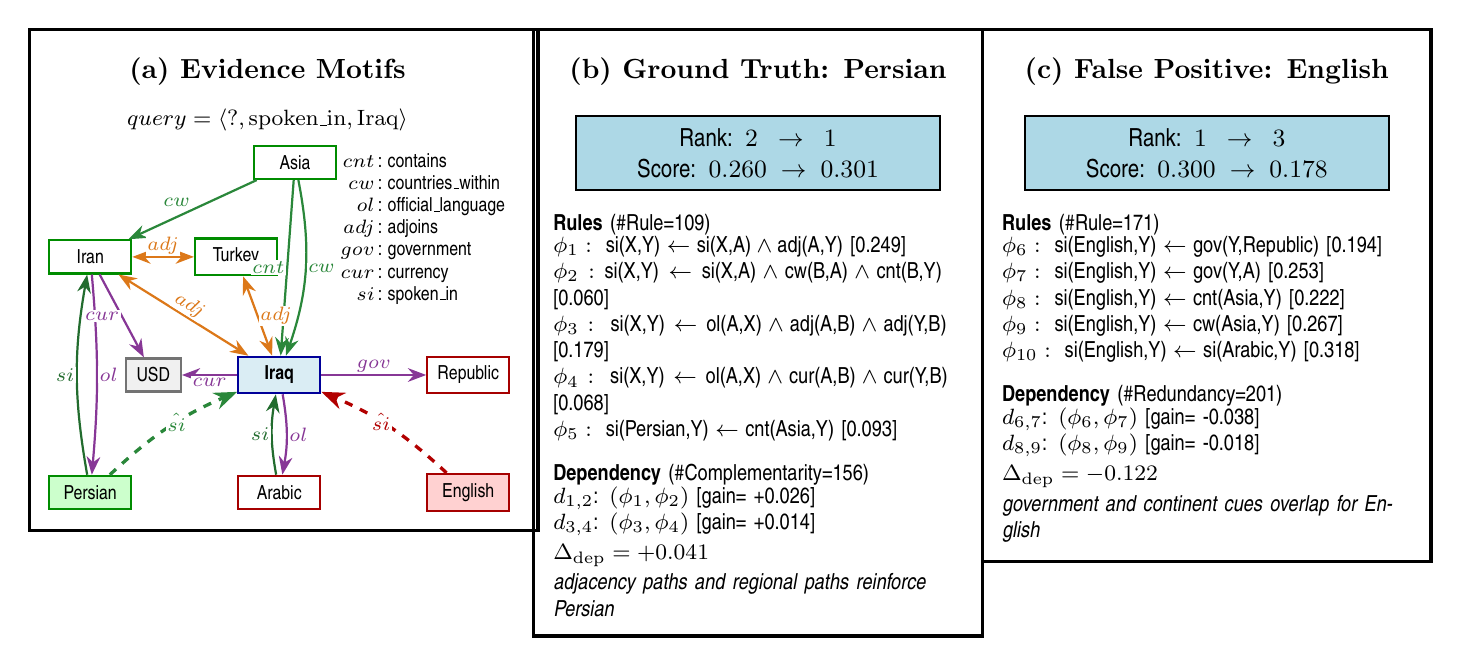
\begin{tikzpicture}[
    node distance=0.22cm,
    box/.style={rectangle, draw, thick, minimum width=2.5cm, minimum height=0.55cm, align=center, font=\fontfamily{phv}\fontseries{c}\selectfont\small},
    title/.style={font=\bfseries\normalsize},
    formula/.style={font=\figbody, align=left},
    section/.style={rectangle, draw=black, very thick, inner sep=2.4mm},
    ent/.style={rectangle, draw, thick, minimum width=1.04cm, minimum height=0.42cm, align=center, font=\fontfamily{phv}\fontseries{c}\selectfont\scriptsize},
    gt/.style={ent, fill=white, draw=green!55!black},
    cone/.style={ent, fill=white, draw=red!65!black},
    aux/.style={ent, fill=lightgray, draw=black!55, minimum width=0.70cm},
    gtfocus/.style={gt, fill=green!20, line width=0.75pt},
    conefocus/.style={cone, fill=red!18, line width=0.75pt},
    qent/.style={ent, fill=lightblue!45, draw=blue!60!black, font=\fontfamily{phv}\fontseries{bc}\selectfont\scriptsize},
    contains/.style={-Stealth, thick, edgegreen},
    official/.style={-Stealth, thick, edgepurple},
    adjoins/.style={Stealth-Stealth, thick, edgeorange},
    spoken/.style={-Stealth, thick, edgegreen!80!black},
    predg/.style={-Stealth, very thick, dashed, edgegreen},
    predr/.style={-Stealth, very thick, dashed, red!70!black},
    elab/.style={font=\fontfamily{phv}\fontseries{c}\selectfont\scriptsize, fill=white, inner sep=0.6pt},
    legend/.style={font=\fontfamily{phv}\fontseries{c}\selectfont\scriptsize, align=left}
]

% ============ (a) Local KG / evidence motifs ============
\node[title] (title-a) at (0,0) {(a) Evidence Motifs};
\node[formula, below=0.05cm of title-a] (query) {$query=\langle ?,\mathrm{spoken\_in},\mathrm{Iraq}\rangle$};

\node[gt] (asia) at (0.35,-1.15) {Asia};
\node[gt] (iran) at (-2.25,-2.35) {Iran};
\node[gt] (turkey) at (-0.4,-2.35) {Turkey};
\node[cone] (republic) at (2.55,-3.85) {Republic};
\node[qent] (iraq) at (0.15,-3.85) {Iraq};
\node[aux] (gdpb) at (-1.45,-3.85) {USD};
\node[gtfocus] (persian) at (-2.25,-5.34) {Persian};
\node[cone] (arabic) at (0.15,-5.34) {Arabic};
\node[conefocus] (english) at (2.55,-5.34) {English};

\node[legend] (kg-legend) at (2,-2) {%
    \begin{tabular}{@{}r@{\,: }l@{}}
    $cnt$ & contains\\
    $cw$ & countries\_within\\
    $ol$ & official\_language\\
    $adj$ & adjoins\\
    $gov$ & government\\
    $cur$ & currency\\
    $si$ & spoken\_in
    \end{tabular}
};

\draw[contains] (asia) -- node[elab,above left] {$cw$} (iran);
\draw[contains] (asia) to[bend right=0] node[elab,left] {$cnt$} (iraq);
\draw[contains] (asia) to[bend left=15] node[elab,right] {$cw$} (iraq);
\draw[spoken] (persian) to[bend left=10] node[elab,left] {$si$} (iran);
\draw[official] (iran) to[bend left=5] node[elab,right] {$ol$} (persian);
\draw[official] (iraq) -- node[elab,above] {$gov$} (republic);
\draw[official] (iran) -- node[elab,left] {$cur$} (gdpb);
\draw[official] (iraq) -- node[elab,below] {$cur$} (gdpb);
\draw[adjoins] (iran) -- node[elab,above,sloped] {$adj$} (iraq);
\draw[adjoins] (iran) -- node[elab,above] {$adj$} (turkey);
\draw[adjoins] (iraq) -- node[elab,right] {$adj$} (turkey);
\draw[official] (iraq) to[bend left=10] node[elab,right] {$ol$} (arabic);
\draw[spoken] (arabic) to[bend left=10] node[elab,left] {$si$} (iraq);
\draw[predg] (persian) to[bend left=10] node[elab,pos=0.56] {$\hat{si}$} (iraq);
\draw[predr] (english) to[bend right=10] node[elab,pos=0.56] {$\hat{si}$} (iraq);

\begin{scope}[on background layer]
\node[section, fit=(title-a)(query)(asia)(iran)(turkey)(republic)(gdpb)(iraq)(persian)(english)(arabic)(kg-legend)] (sec-a) {};
\end{scope}

% ============ (b) GT Persian ============
\node[title] (title-b) at (6.23,0) {(b) Ground Truth: Persian};

\node[box, fill=lightblue, below=0.25cm of title-b, text width=4.3cm, inner sep=1.6mm] (gt-score) {
    Rank: $2 \to 1$ \\
    Score: $0.260 \to 0.301$
};

\node[formula, below=0.28cm of gt-score, text width=5.20cm, inner sep=0mm] (gt-rules) {
    \textbf{Rules} (\#Rule=109)\\[-0.5mm]
    $\phi_1:\ \text{si(X,Y)}\leftarrow \text{si(X,A)}\wedge \text{adj(A,Y)}$ [0.249]\\
    $\phi_2:\text{si(X,Y)}\leftarrow \text{si(X,A)}\wedge \text{cw(B,A)}\wedge \text{cnt(B,Y)}$ [0.060]\\
    $\phi_3:\ \text{si(X,Y)}\leftarrow \text{ol(A,X)}\wedge \text{adj(A,B)}\wedge \text{adj(Y,B)}$ [0.179]\\
    $\phi_4:\ \text{si(X,Y)}\leftarrow \text{ol(A,X)}\wedge \text{cur(A,B)}\wedge \text{cur(Y,B)}$ [0.068]\\
    $\phi_5:\ \text{si(Persian,Y)}\leftarrow \text{cnt(Asia,Y)}$ [0.093]
};

\node[formula, below=0.28cm of gt-rules, text width=5.20cm, inner sep=0mm] (gt-dep) {
    \textbf{Dependency} (\#Complementarity=156)\\[-0.5mm]
    $d_{1,2}$: $(\phi_1, \phi_2)$ [gain= +0.026]\\
    $d_{3,4}$: $(\phi_3, \phi_4)$ [gain= +0.014]\\[0.5mm]
    $\Delta_{\rm dep}=+0.041$\\[0.5mm]
    \textit{adjacency paths and regional paths reinforce Persian}
};

\begin{scope}[on background layer]
\node[section, fit=(title-b)(gt-score)(gt-rules)(gt-dep), inner sep=2.4mm] (sec-b) {};
\end{scope}

% ============ (c) FP English ============
\node[title] (title-c) at (11.93,0) {(c) False Positive: English};

\node[box, fill=lightblue, below=0.25cm of title-c, text width=4.3cm, inner sep=1.6mm] (fp-score) {
    Rank: $1 \to 3$ \\
    Score: $0.300 \to 0.178$
};

\node[formula, below=0.28cm of fp-score, text width=5.20cm, inner sep=0mm] (fp-rules) {
    \textbf{Rules} (\#Rule=171)\\[-0.5mm]
    $\phi_6:\ \text{si(English,Y)}\leftarrow \text{gov(Y,Republic)}$ [0.194]\\
    $\phi_7:\ \text{si(English,Y)}\leftarrow \text{gov(Y,A)}$ [0.253]\\
    $\phi_8:\ \text{si(English,Y)}\leftarrow \text{cnt(Asia,Y)}$ [0.222]\\
    $\phi_9:\ \text{si(English,Y)}\leftarrow \text{cw(Asia,Y)}$ [0.267]\\
    $\phi_{10}:\ \text{si(English,Y)}\leftarrow \text{si(Arabic,Y)}$ [0.318]
};

\node[formula, below=0.28cm of fp-rules, text width=5.20cm, inner sep=0mm] (fp-dep) {
    \textbf{Dependency} (\#Redundancy=201)\\[-0.5mm]
    $d_{6,7}$: $(\phi_6, \phi_7)$ [gain= -0.038]\\
    $d_{8,9}$: $(\phi_8, \phi_9)$ [gain= -0.018]\\[0.5mm]
    $\Delta_{\rm dep}=-0.122$\\[0.5mm]
    \textit{government and continent cues overlap for English}
};

\begin{scope}[on background layer]
\node[section, fit=(title-c)(fp-score)(fp-rules)(fp-dep), inner sep=2.4mm] (sec-c) {};
\end{scope}

\end{tikzpicture}
\end{document}
